\section{Beyond the Standard Model}
Many beyond the SM (BSM) theories have been proposed to address the issues discussed in Section~\ref{sm_status}. Theories such as large extra dimensions address the unnatural Higgs boson mass by allowing gravity to spread across more than three spatial dimensions, which lowers $M_P$ and therefore the size of the Higgs boson mass corrections~\cite{add}. Other theories posit new symmetries that protect the Higgs boson mass from large corrections. The following section explains supersymmetry, which protects the Higgs boson mass with a new symmetry between bosons and fermions.

\subsection{Supersymmetry}
\label{susy}
Supersymmetry (SUSY) introduces a new symmetry in which every SM particle fits into a larger multiplet with an inherent symmetry between bosons and fermions. In its simplest form, SUSY predicts one new boson for every SM fermion, one new fermion for every SM boson, and one new Higgs doublet. The increase in particle multiplicity necessitates a new naming convention: the spin-0 superpartners of the SM fermions are called sfermions (e.g. sleptons or squarks) while the spin-$\frac{1}{2}$ superpartners to the SM bosons add ``ino" to the end of their SM counterpart (e.g. Higgsino or wino).

When calculating contributions to the Higgs boson mass from loop diagrams, one finds that fermion loops differ in sign from boson loops, which means that in SUSY every bosonic correction to the Higgs boson mass is cancelled by a fermionic correction and vice versa. If SUSY were an exact symmetry of nature, the cancellation would be perfect, and the observed Higgs boson mass would match the bare Higgs boson mass exactly~\cite{susy_primer}. Figure~\ref{higgs_top_stop_corrections} shows a sample leading-order cancellation.

\begin{figure}[hbtp]
\centering
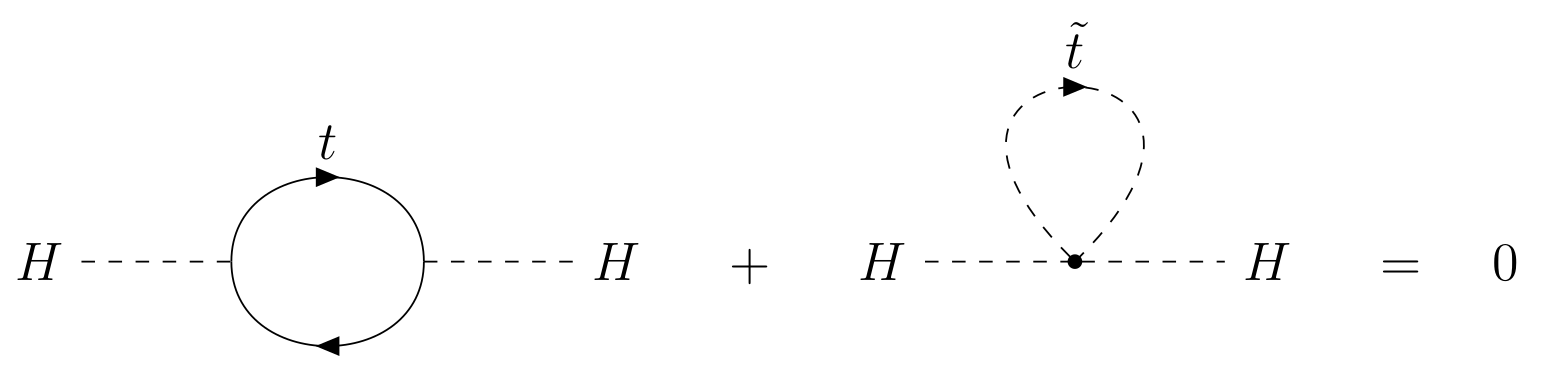
\includegraphics[scale=0.2]{figures/intro/higgs_top_stop_corrections.png}
\caption{Corrections to the Higgs boson mass from the top quark (left) and top squark (right) cancel in exact SUSY. The top quark and top squark contributions are enhanced by the large top--Higgs coupling.}
\label{higgs_top_stop_corrections}
\end{figure}

Exact SUSY also requires that SUSY particles have the same mass as their SM counterparts, so the uniformly null results in collider searches imply that if SUSY exists, it must be a broken symmetry. In broken SUSY, the diagrams in Fig.~\ref{higgs_top_stop_corrections} no longer exactly cancel. Instead, the resulting correction is proportional to the mass of the top squark~\cite{craig_susy_run1}, which means that broken SUSY can still resolve the naturalness problem if the masses of the SUSY particles that correct the Higgs boson mass are themselves approximately at the weak scale (say $\mathcal{O}(\SI{250}{\GeV}$)). Many natural SUSY scenarios are therefore excluded as collider experiments set increasingly large lower bounds on SUSY particle masses. Figure~\ref{cms_susy_summary}, for example, shows that the exclusion bounds on top squark and gluino masses extend above \SI{1}{\TeV} in several recent CMS analyses. 

\begin{figure}
\centering
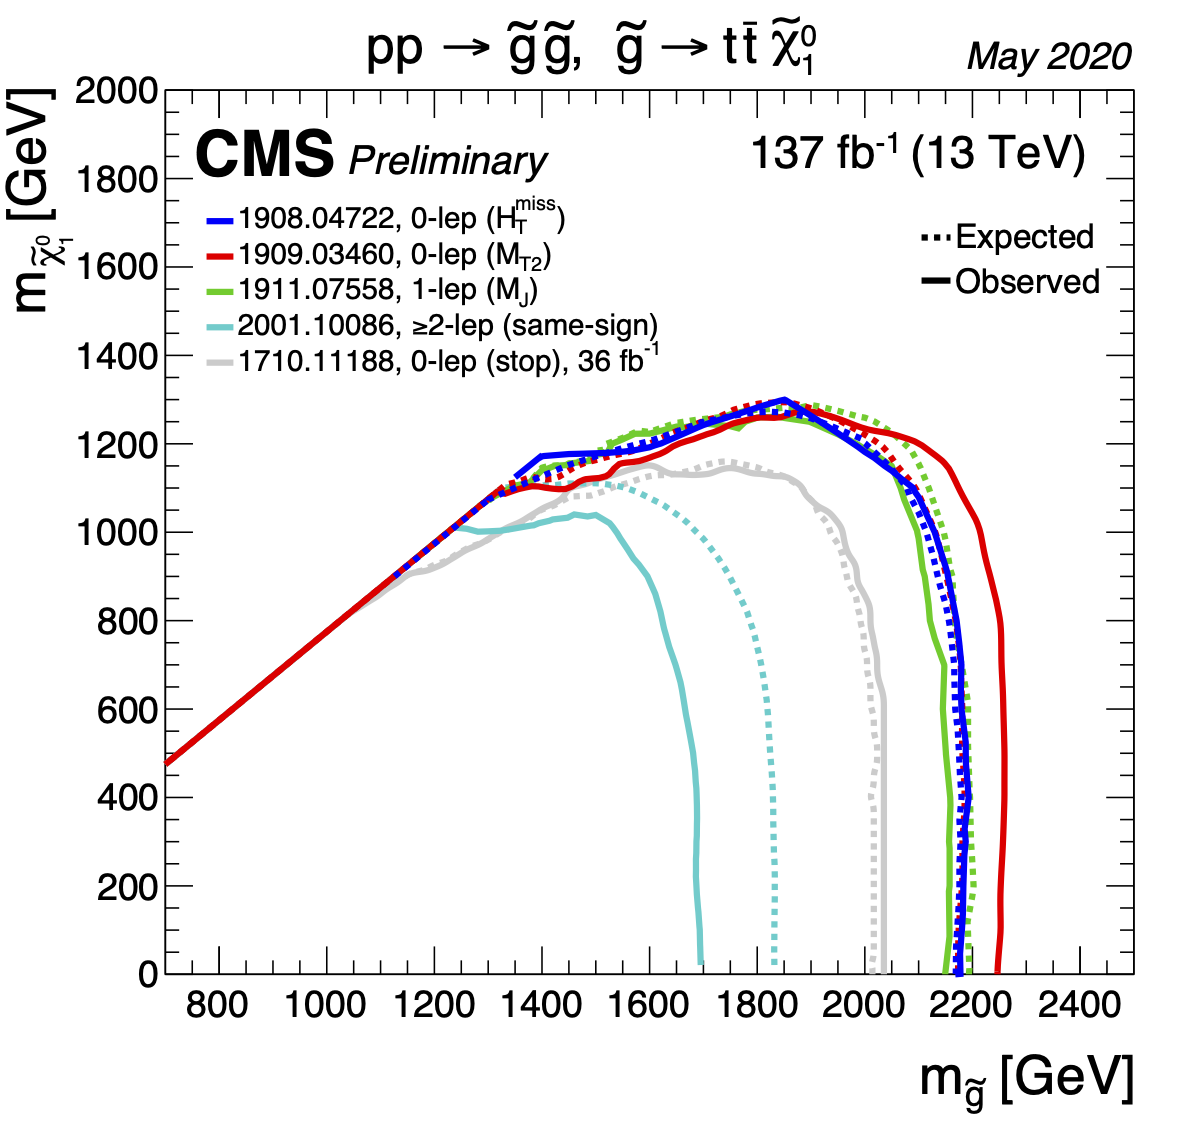
\includegraphics[width=0.45\textwidth]{figures/intro/gluino_mass_limits.png}
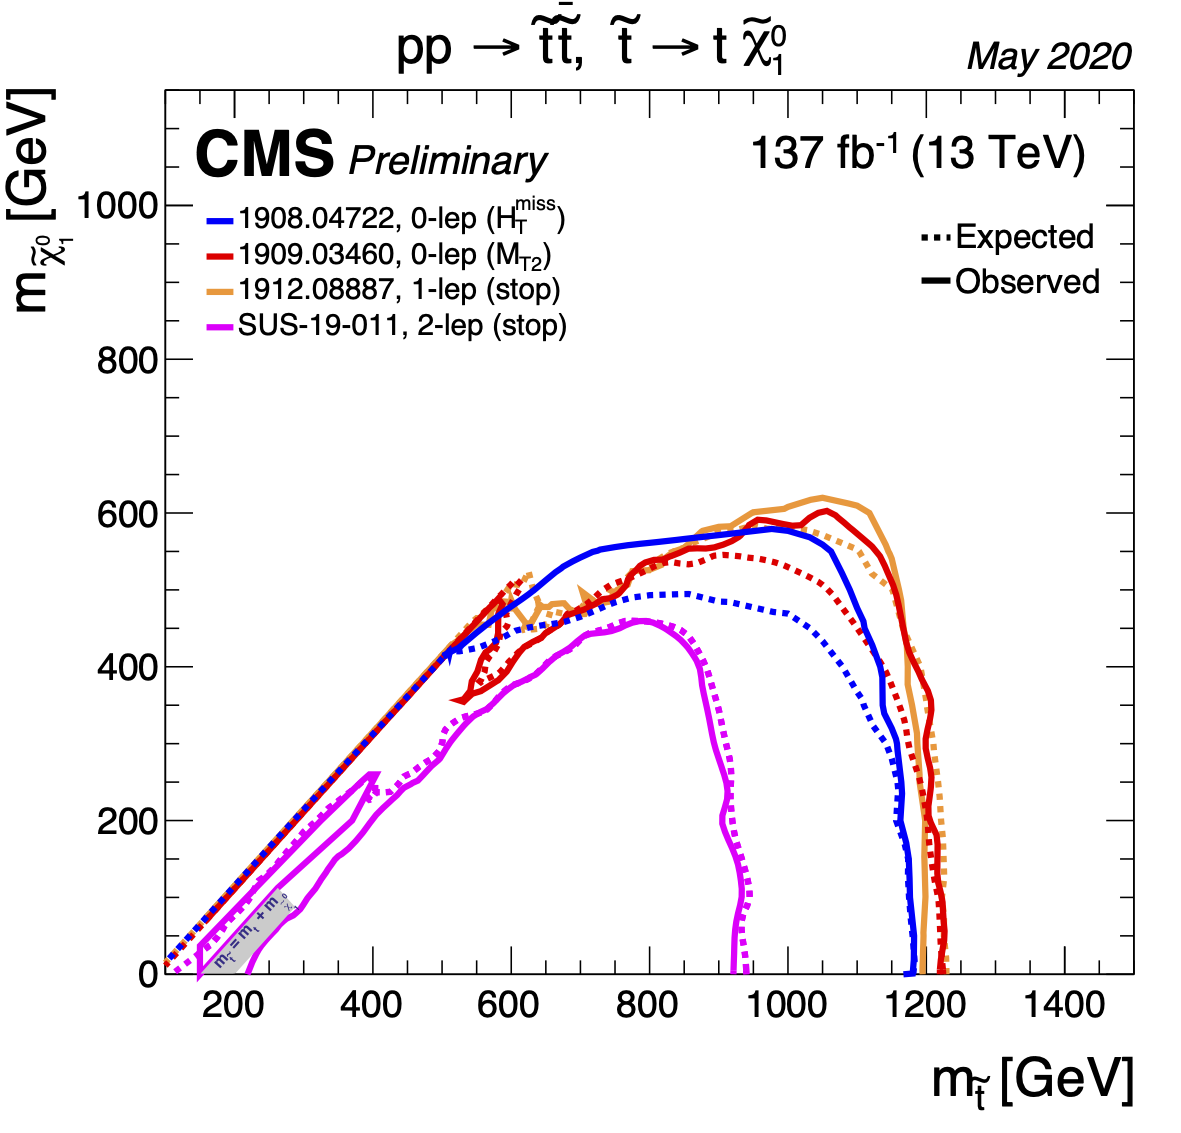
\includegraphics[width=0.45\textwidth]{figures/intro/stop_mass_limits.png}
\caption{Mass limits at \SI{95}{\percent} CL for a simplified model of gluino pair production with gluino decays to pairs of top quarks and the LSP (left) and top squark pair production with squark decays to a top quark and the LSP (right) from several CMS analyses~\cite{cms_susy_public_results}.}
\label{cms_susy_summary}
\end{figure}

As the available natural SUSY parameter space is further constricted, it is important to investigate signatures of new physics that conventional analyses may be missing. One possibility, new long-lived particles, is presented in the following section.

\fxnote{mention gauge unification, dark matter candidate, etc?}

\subsection{Long-lived particles}
\label{llps}
In the context of collider physics, long-lived particles (LLPs) are particles whose lifetimes are such that they decay a measurable distance from the collision point. This category includes everything from particles that decay less than \SI{1}{\mm} away from the collision to particles that propagate through the entire detector. As shown in Fig~\ref{sm_llps}, long-lived particles are common in the SM.

\begin{figure}[hbtp]
\centering
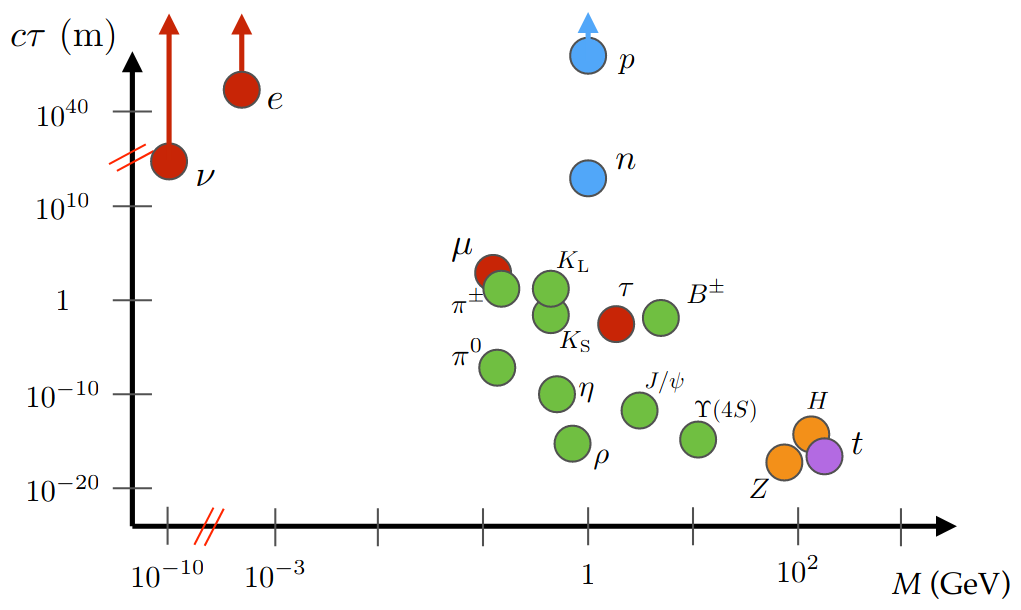
\includegraphics[scale=0.4]{figures/intro/sm_llps.png}
\caption{Masses and proper decay lengths of many Standard Model particles. Particles with proper decay lengths above approximately \SI{e-4}{\m} will be noticeably long-lived in collider detectors such as CMS.\fxnote{cite https://indico.cern.ch/event/607314/contributions/2542308/attachments/1447888/2231430/LHC-LLP_Shuve.pdf}}
\label{sm_llps}
\end{figure}

Long-lived SM particles arise from several mechanisms. First, symmetries such as charge and baryon number conservation ensure that particles such as electrons and protons are absolutely stable. Second, small coupling constants and highly virtual intermediate states decrease the decay rate of particles such as muons, whose \SI{2.2}{\us} lifetime is the product of a weak decay through a virtual $W$ boson (the $W$ boson mass is about \num{760} times that of the muon). Finally, limited decay phase space increases the lifetime of particles such as the neutron, whose decay into a proton, an electron, and an electron neutrino is slowed by the near mass degeneracy of the neutron and the proton. The mass difference between the neutron and its decay products is less than \SI{1}{\MeV}. The muon and neutron decays are diagrammed in Fig.~\ref{neutron_muon_decays}.

\begin{figure}
\centering
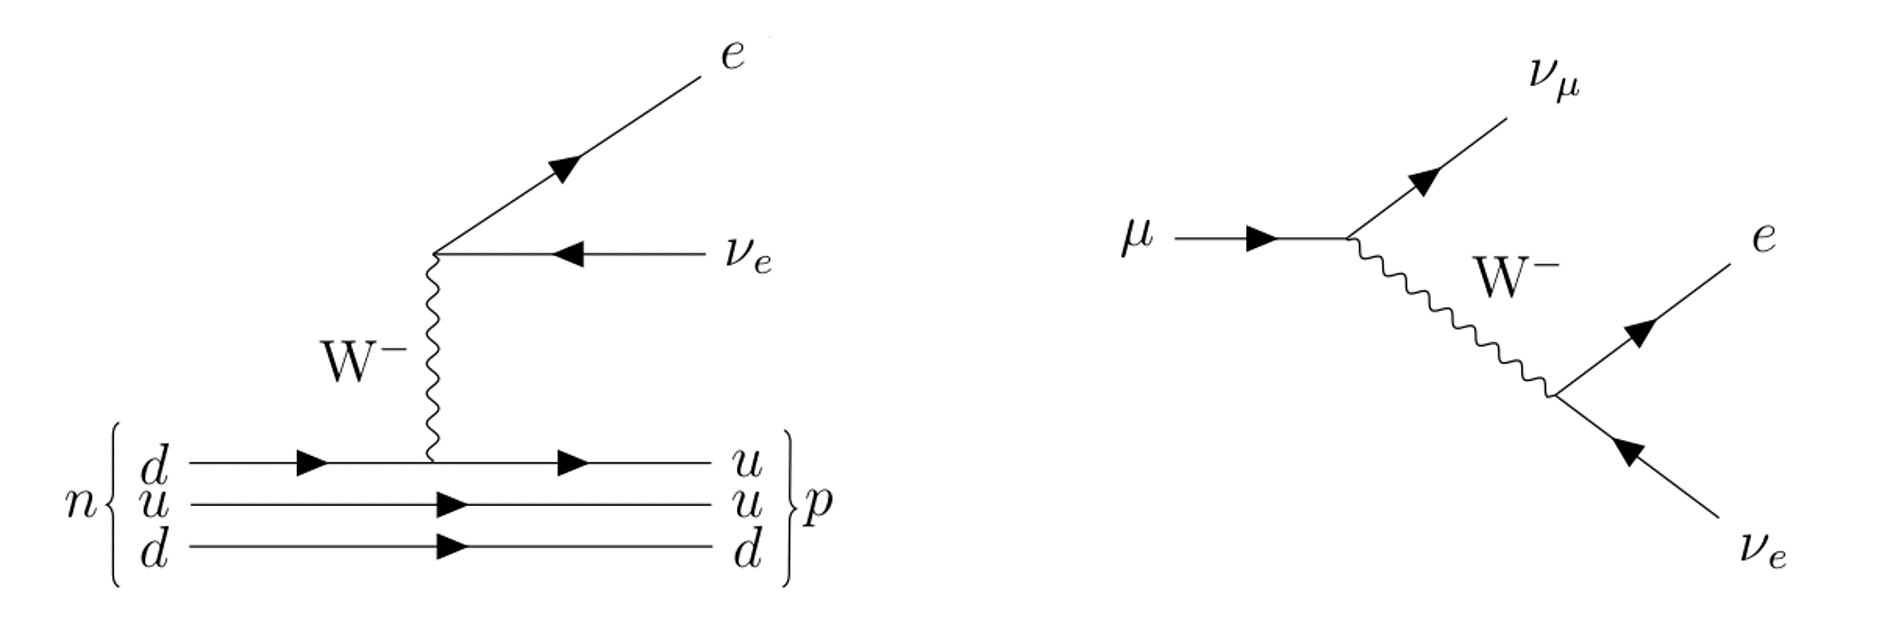
\includegraphics[width=0.9\textwidth]{figures/intro/neutron_muon_decays.pdf}
\caption{Long-lived decays of the neutron (left) and muon (right).}
\label{neutron_muon_decays}
\end{figure}

In BSM physics, the same fundamental mechanisms could very well produce new long-lived particles. Many SUSY scenarios, for example, introduce a symmetry known as R parity that prevents proton decay. In models with exact R-parity conservation, SM particles are assigned R-parity \num{+1} and SUSY particles are assigned R-parity \num{-1}. Conserving the product of R-parity at each vertex has two phenomenological consequences: SUSY particles must be produced in pairs, and the lightest SUSY particle (LSP) must be absolutely stable. A neutral, weakly interacting LSP would therefore pass through most detectors (including the CMS detector described in Section~\ref{cms}) without interacting. The resulting momentum imbalance is a standard signature in many SUSY searches~\cite{pdg_2020}.

On the other hand, SUSY models with weakly coupled R-parity violating (RPV) terms produce long-lived but not perfectly stable LSPs. The following section will give a detailed overview of one such model. A similar situation arises in gauge-mediated SUSY breaking models where the gravitino\fxnote{I never defined the graviton} is the LSP. The strength of the coupling between the next-to-LSP (NLSP) and the gravitino is inversely proportional to the energy scale at which SUSY is broken. A high SUSY breaking scale therefore suppresses the NLSP decay rate, making it long lived~\cite{liu_2015}.

LLPs also arise from particular SUSY mass spectra. Models in the Split SUSY paradigm, for example, propose that the spin-0 SUSY particles are significantly more massive than the spin-$\frac{1}{2}$ SUSY particles. In these models, the gluino becomes long lived when its decay to two quarks and a neutral spin-$\frac{1}{2}$ SUSY particle is suppressed by a highly virtual intermediate squark~\cite{split_susy_colliders}. Other SUSY models produce long-lived particles by limiting decay phase space. Some anomaly-mediated SUSY breaking models, for example, predict that the NLSP and LSP are nearly degenerate in mass. Just like the neutron decaying into a proton, the lack of available phase space suppresses the decay and produces a long-lived NLSP~\cite{amsb_at_lhc}.

In summary, LLPs are a general feature of the SM, and it is reasonable to assume that the same mechanisms that produce SM LLPs will also manifest in BSM physics. The following subsection gives an overview of the phenomenology of the SUSY model most relevant to the analysis presented in Chapter~\ref{displaced_leptons}, while the experimental details of this model and LLP searches at the LHC will be saved until after presenting the LHC and CMS experiment in Chapter~\ref{lhc_and_cms}.

\subsection{Displaced supersymmetry}
\label{displaced_susy}
As mentioned in Section~\ref{susy}, weak-scale SUSY has the potential to explain the seemingly unnatural observed value of the Higgs boson mass. With this appealing outcome in mind, experimental physicists have been searching for signs of SUSY in high-energy particle collisions for the last few decades. In particular, searches at the Large Hadron Collider, where the \num{7}, \num{8}, and \SI{13}{\TeV} proton-proton collisions could potentially be producing SUSY particles with masses above \SI{1}{\TeV}\fxnote{cite susy production xs? pdg figure 90.1 is nice}, are actively excluding large swaths of the natural SUSY parameter space\fxnote{cite something}. By examining the common assumptions behind a majority of these searches, the proponents of the Displaced SUSY model find an approach that avoids proton decay constraints while naturally producing long-lived SUSY particles that would be undetected by most collider searches~\cite{displaced_susy}.

Displaced SUSY is an RPV SUSY model that respects proton lifetime constraints by allowing terms that violate lepton number but not baryon number. The Minimal Supersymmetric Standard Model, which is a simple supersymmetric extension of the SM, allows the following baryon and lepton violating operators:
\begin{equation}
    \label{lepton_baryon_violating_terms}
    \frac{1}{2}\lambda''_{ijk}U_{i}D_{j}D_{k},\ \frac{1}{2}\lambda_{ijk}L_{i}L_{j}E_{k},\  \lambda'_{ijk}L_{i}Q_{j}D_{k},\  \epsilon_{i}L_{i}H_{u} 
\end{equation}
where the first term violates baryon number and the remaining terms violate lepton number. The i, j, and k indices run over the three generations of fermions and $U$, $D$, $L$, $E$, $Q$, and $H$ refer to the SUSY multiplets whose SM components are right-handed up-type quarks, right-handed down-type quarks, left-handed leptons, right-handed leptons, left-handed quarks, and Higgs bosons, respectively~\cite{susy_primer}. Most SUSY models introduce R-parity to forbid all of these terms and therefore disallow proton decay, but this approach may be overkill: separately conserving either lepton number or baryon number is sufficient to prevent proton decay.

Such a situation can arise naturally if a gauge-unifying, R-parity-conserving $SU(5)$ theory exists at high energies but is broken at lower energies~\cite{hall_suzuki_rpv}. In this scenario, the baryon-number-violating terms are suppressed and mixing between $L$ and $H$ becomes possible. The final term in expression~\eqref{lepton_baryon_violating_terms} then dominates, and we are left with the following lepton-number-violating terms after rotating to the mass basis\fxnote{learn this better}:
\begin{equation}
    \label{displaced_susy_terms}
    \epsilon_{i}y^{d}_{jk}L_{i}Q_{j}D_{k},\ \epsilon_{i}y^{e}_{jk}L_{i}L_{j}E_{k} 
\end{equation}
where the $\epsilon$ factors are lepton-Higgs mixing angles and the $y$ factors are the Yukawa coupling constants associated with the interactions between the fermions and the SM Higgs field. Because these $y$ factors are proportional to fermion mass, the lepton-violating processes will favor third-generation fermions.
\fxnote{mention tree-level neutrino masses somewhere?}

The dimensionless lepton-Higgs mixing angles are protected by the custodial R-parity conservation of the higher-energy theory and will therefore naturally be small. Just as in the SM, these small coupling constants can lead to macroscopic SUSY particle lifetimes that would evade most collider searches. In particular, long-lived LSP squarks can decay to a quark and charged lepton though a displaced vertex, as in Fig.~\ref{stop_to_lb}.

\begin{figure}
\centering
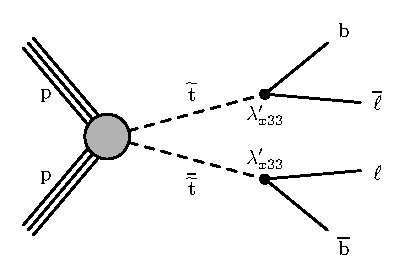
\includegraphics[width=0.5\textwidth]{figures/intro/stopToLB.pdf}
\caption{Pair-produced top squarks that each decay to a bottom quark and a lepton through an R-parity-violating $LQD$ vertex.}
\label{stop_to_lb}
\end{figure}

The unique experimental signature of processes such as the one shown in Fig.~\ref{stop_to_lb} is a major motivating factor behind the analysis presented in Chapter~\ref{displaced_leptons}. The particular experimental consequences of such processes will be further explored in that context.

\pagebreak